\documentclass[11pt]{article}

\usepackage{graphicx, subcaption, amsfonts, amsmath, amsthm, empheq, setspace, lscape}
\usepackage[top=1in, bottom=1in, left=1in, right=1in]{geometry}

% define some commands
% command to box formula
\newcommand*\widefbox[1]{\fbox{\hspace{2em}#1\hspace{2em}}}
\newlength\dlf
\newcommand\alignedbox[2]{
  % Argument #1 = before & if there were no box (lhs)
  % Argument #2 = after & if there were no box (rhs)
  &  % Alignment sign of the line
  {
    \settowidth\dlf{$\displaystyle #1$}  
    % The width of \dlf is the width of the lhs, with a displaystyle font
    \addtolength\dlf{\fboxsep+\fboxrule}  
    % Add to it the distance to the box, and the width of the line of the box
    \hspace{-\dlf}  
    % Move everything dlf units to the left, so that & #1 #2 is aligned under #1 & #2
    \boxed{#1 #2}
    % Put a box around lhs and rhs
  }
}

\newcommand\ER{Erd\H{o}s-R'{e}nyi}
\newcommand{\Forall}{\; \forall \;}
\DeclareMathOperator*{\argmin}{\arg\!\min}

% change captions
\captionsetup{width=0.8\textwidth}
\captionsetup{labelformat=empty,labelsep=none}

% set paragraph indent length
\setlength\parindent{0pt}

% set folder for imported graphics
\graphicspath{ {./figs/} }

\title{Overview of sloppy models}

\begin{document}
\maketitle

Below is a brief overview of the various models we could employ to display different varieties of sloppiness.

\section{Singularly perturbed}

The only purely singularly perturbed problem is a basic, reversible reaction mechanism involving three components: A, B and C.

\subsection{ABC Reaction}

The mechanism is given by

\begin{align*}
  A \xrightleftharpoons[k_{-1}]{k_1} B, \; B \xrightarrow[]{k_2} C
\end{align*}

under the assumption that species $B$ is in quasi equilibrium. This requires

\begin{align*}
  \frac{dC_B}{dt} &= k_1 C_A - (k_{-1} + k_2) C_B = 0 \\
  &\rightarrow C_B = C_A \frac{k_1}{k_{-1} + k_2}
\end{align*}

leading to the analytical, QSSA solution for $C_C$

\begin{align*}
  C_C = C_{A_0}(1 - e^{-\frac{k_1 k_2}{k_{-1} + k_2} t})
\end{align*}

Here we see the effective parameter

\begin{align*}
  k_{eff} = \frac{k_1 k_2}{k_{-1} + k_2}
\end{align*}

will create nonlinear level sets in parameter space instead of simple planes.

as shown below, along with DMAPS parameterization of the sloppy parameter set.

\begin{figure}[htbp]
  \centering
  \includegraphics[width=\linewidth]{abc-dataset}
  \caption{Dataset of sloppy parameter combinations}
\end{figure}

As expected, it maps out a two-dimensional surface in parameter space over which $k_{eff}$ is nearly constant ($k_{eff} \in (0.4, 1.0)$ in the dataset above).

When DMAPS was applied, the first two eigenvectors parameterized the surface as hoped. This is shown in the two figures below.

\begin{figure}[htbp]
  \centering
  \includegraphics[width=\linewidth]{abc-dmap1}
  \caption{Coloring the dataset by the first DMAP parameter/coordinate value}
\end{figure}

\begin{figure}[htbp]
  \centering
  \includegraphics[width=\linewidth]{abc-dmap2}
  \caption{Coloring the dataset by the second DMAP parameter/coordinate value}
\end{figure}

\section{Regularly perturbed}

Here we have the Michaelis Menten system. Although it, too, is singularly perturbed, the parameter transformation we apply reveals two \textit{regular} perturbation paramters $\kappa$ and $\epsilon$.

\subsection{Michaelis Menten}

This is another reaction system which we apply the QSSA to, but in this case we transform the bare parameters into 

\begin{align*}
  V_M &= k_2 E_T \\
  K_M &= \frac{k_{-1} + k_2}{k_1} \\
  \kappa &= \frac{k_{-1}}{k_2} \\
  \epsilon &= \frac{E_T}{S_T + K_M} \\
\end{align*}

in which $\kappa$ and $\epsilon$ drop out of the leading dynamics and are thus sloppy. However, these parameter combinations \textbf{do not} yield nonlinear contours in the original parameter space as desired. The figure below shows the ellipsoidal contour produced by this system in the $K_M$, $V_M$ and $S_T$ parameter space, combinations of which are also sloppy in certain regimes.

\begin{figure}[htbp]
  \centering
  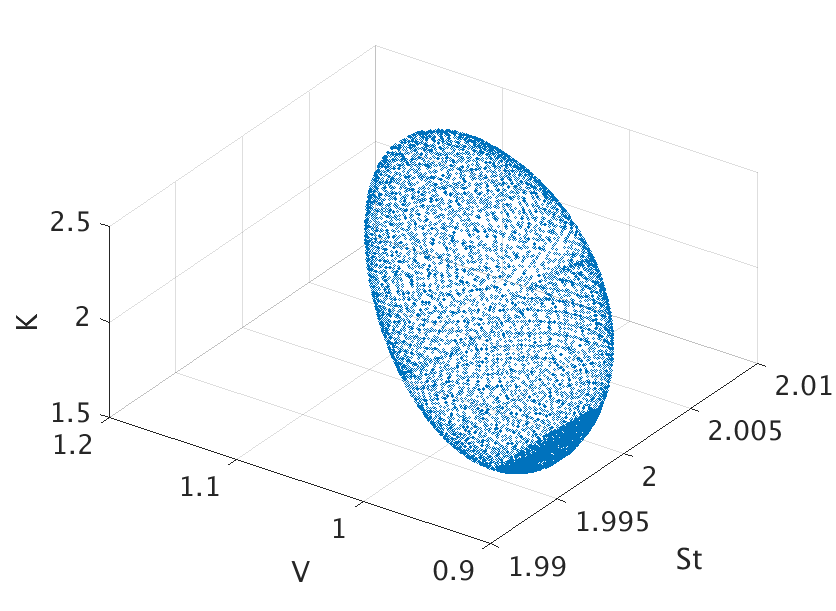
\includegraphics[width=\linewidth]{k-v-st-contour}
  \caption{Ellipsoidal contour of Michaelis Menten system in $K_M$, $V_M$ and $S_T$ parameter space.}
\end{figure}

\section{Singularly and regularly perturbed, sloppy initial conditions}

Here we turn to Antonios' model which includes all varieties of sloppiness we wish to show: singular and regular perturbation parameters and sloppy initial conditions. This system is ideal for a nonlinear transformation of parameters.

\subsection{Antonios' Model}

We start with the linear ODEs

\begin{align*}
  X &= -\lambda X \\
  \epsilon Y &= -Y
\end{align*}

and then transform it into nonlinear $(x, y)$ via 

\begin{align*}
  x &= X + \phi(y) \\
  y &= Y + \mu(x) \\
\end{align*}

We are free to choose $\phi(y)$ and $\mu(x)$, which control the shape of the fast and slow manifold, respectively. Thus, if we set $\mu = a x^2$ and $\phi = b y^2$ we find parabolic slow and fast manifolds, and additionally we've introduced a sloppy regular perturbation parameter $b$. Additionally, initial conditions lying along a given fast manifold will be sloppy. Sloppiness in $\epsilon$/$\lambda$, $a$/$b$ and $x_0$/$y_0$ are shown in the three figures below.

\begin{figure}[htbp]
  \centering
  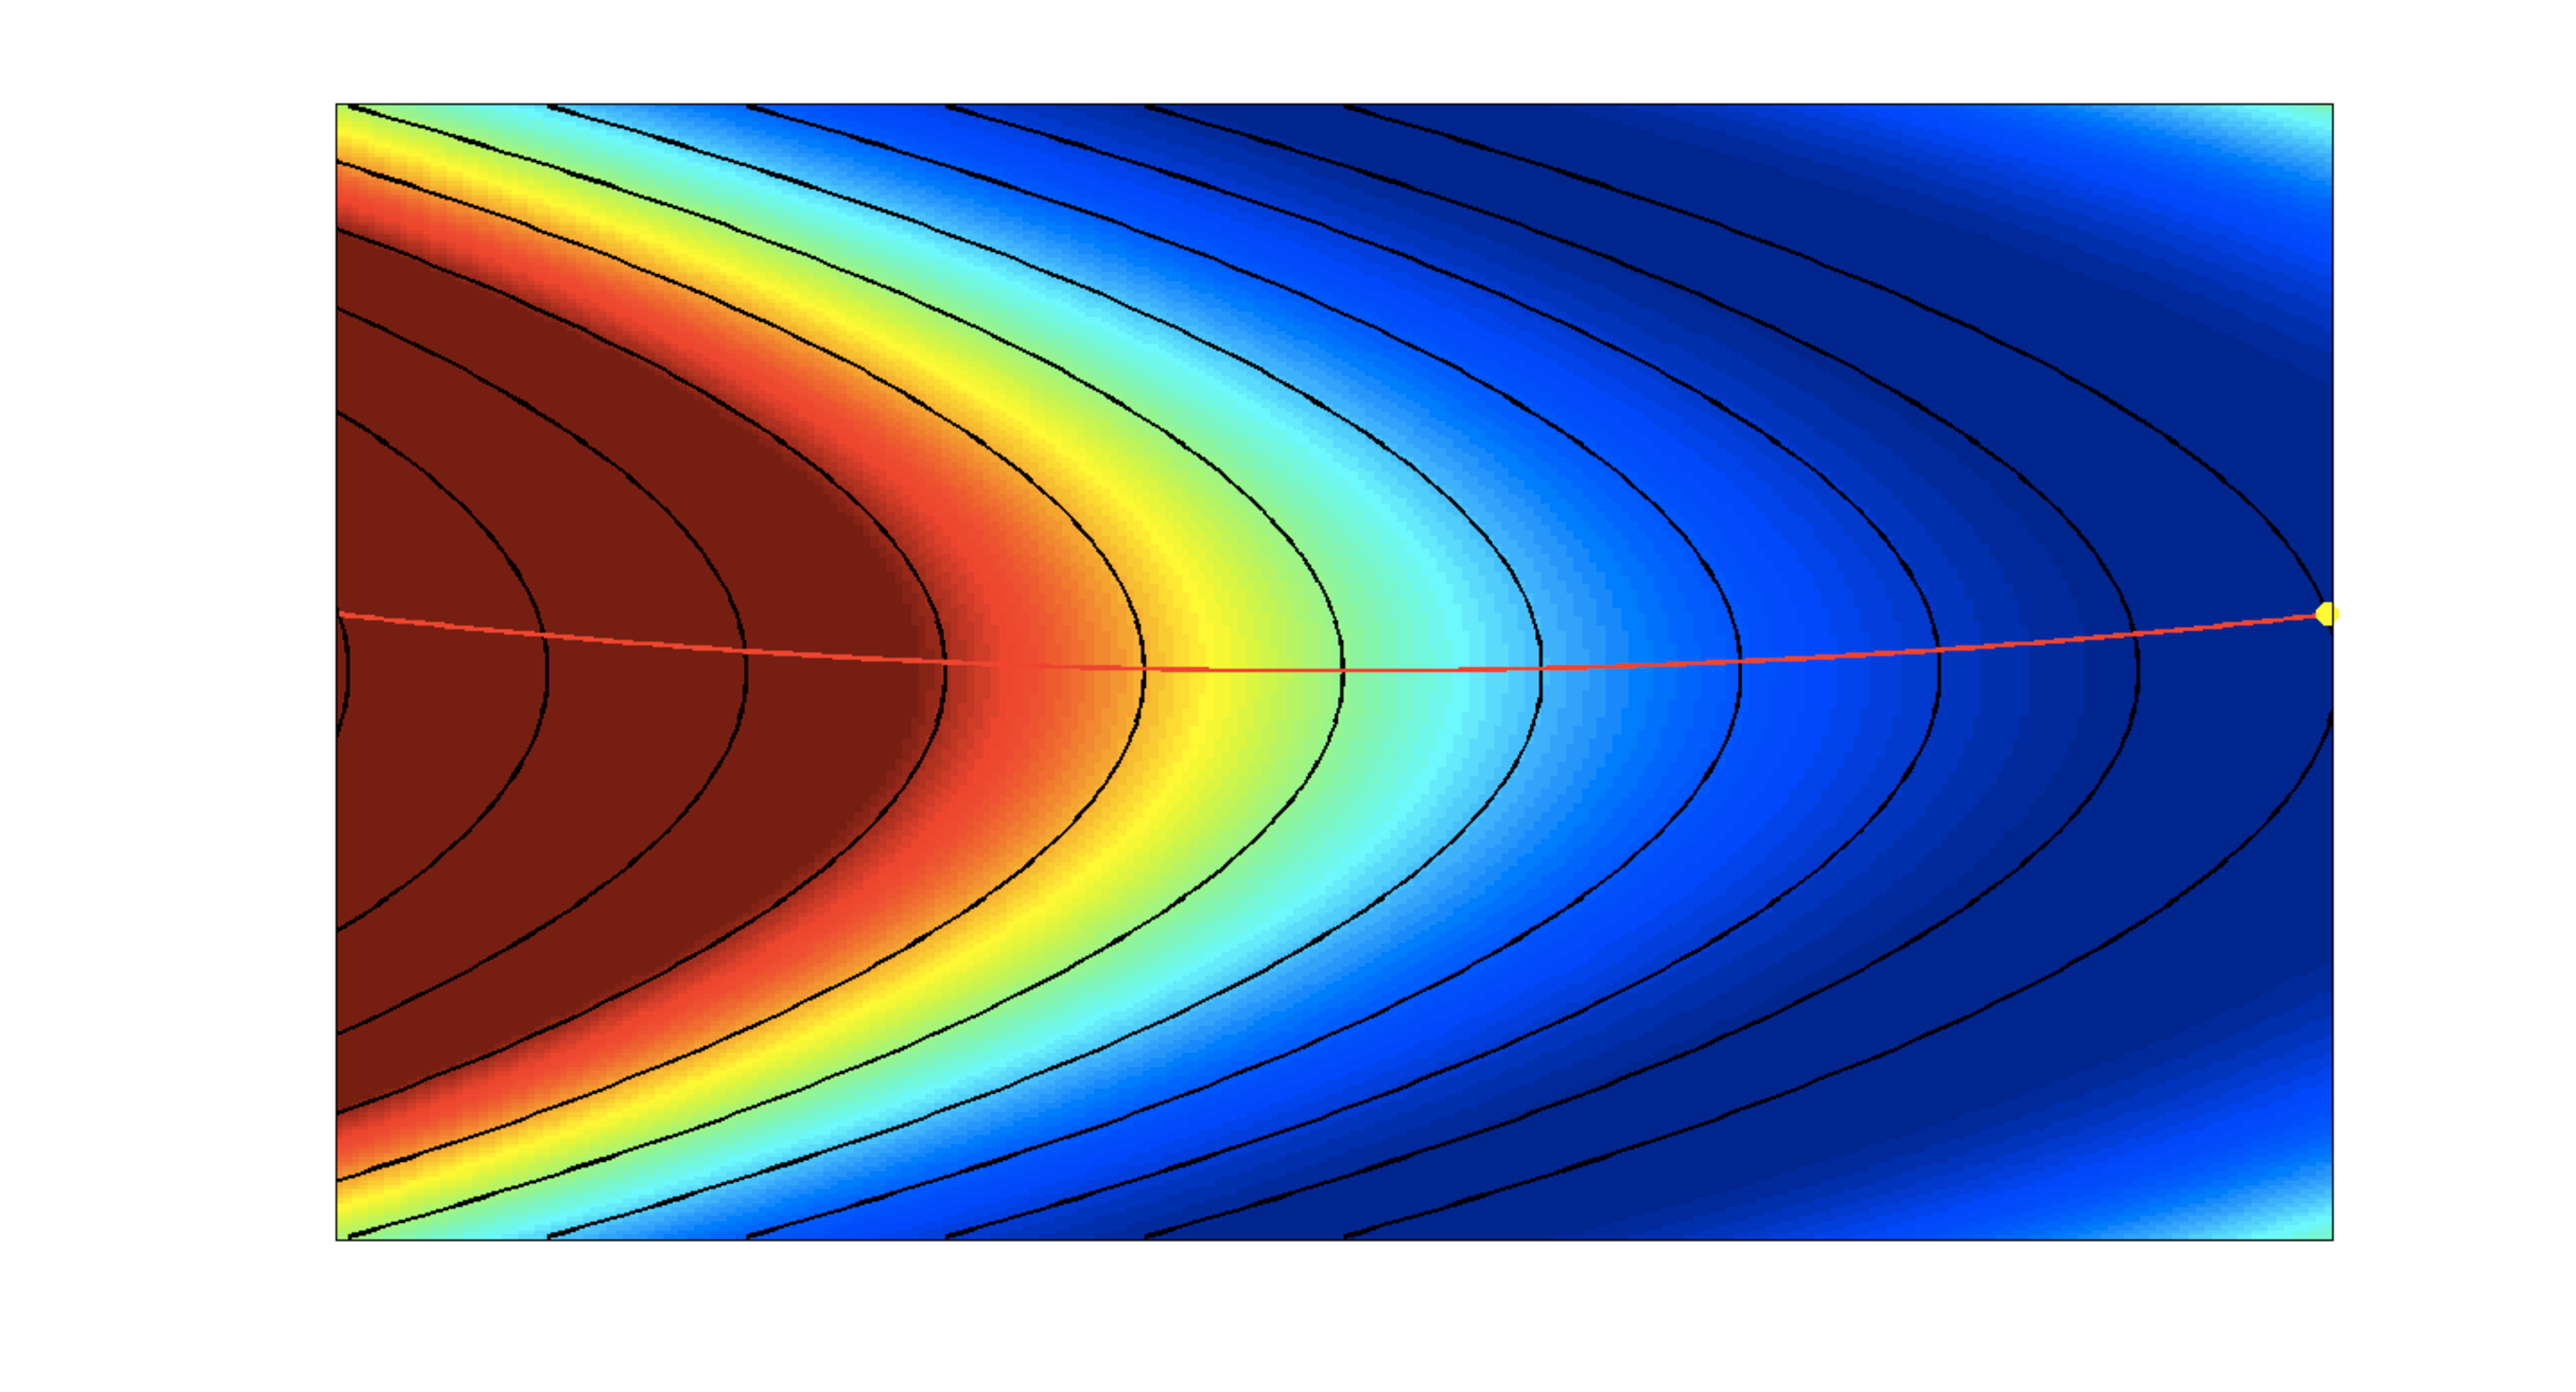
\includegraphics[width=\linewidth]{zagaris-ic-contours}
  \caption{$x_0$/$y_0$ plane colored by objective function value. The contours follow the fast manifold $x=y^2$.}
\end{figure}

\begin{figure}[htbp]
  \centering
  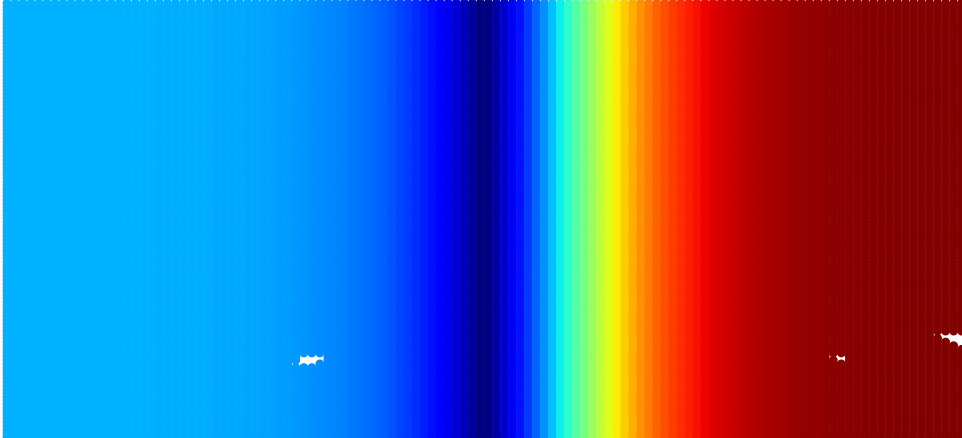
\includegraphics[width=\linewidth]{zagaris-le-contours}
  \caption{$\epsilon$/$\lambda$ plane colored by objective function value. Contours follow lines of constant $\epsilon$.}
\end{figure}

\begin{figure}[htbp]
  \centering
  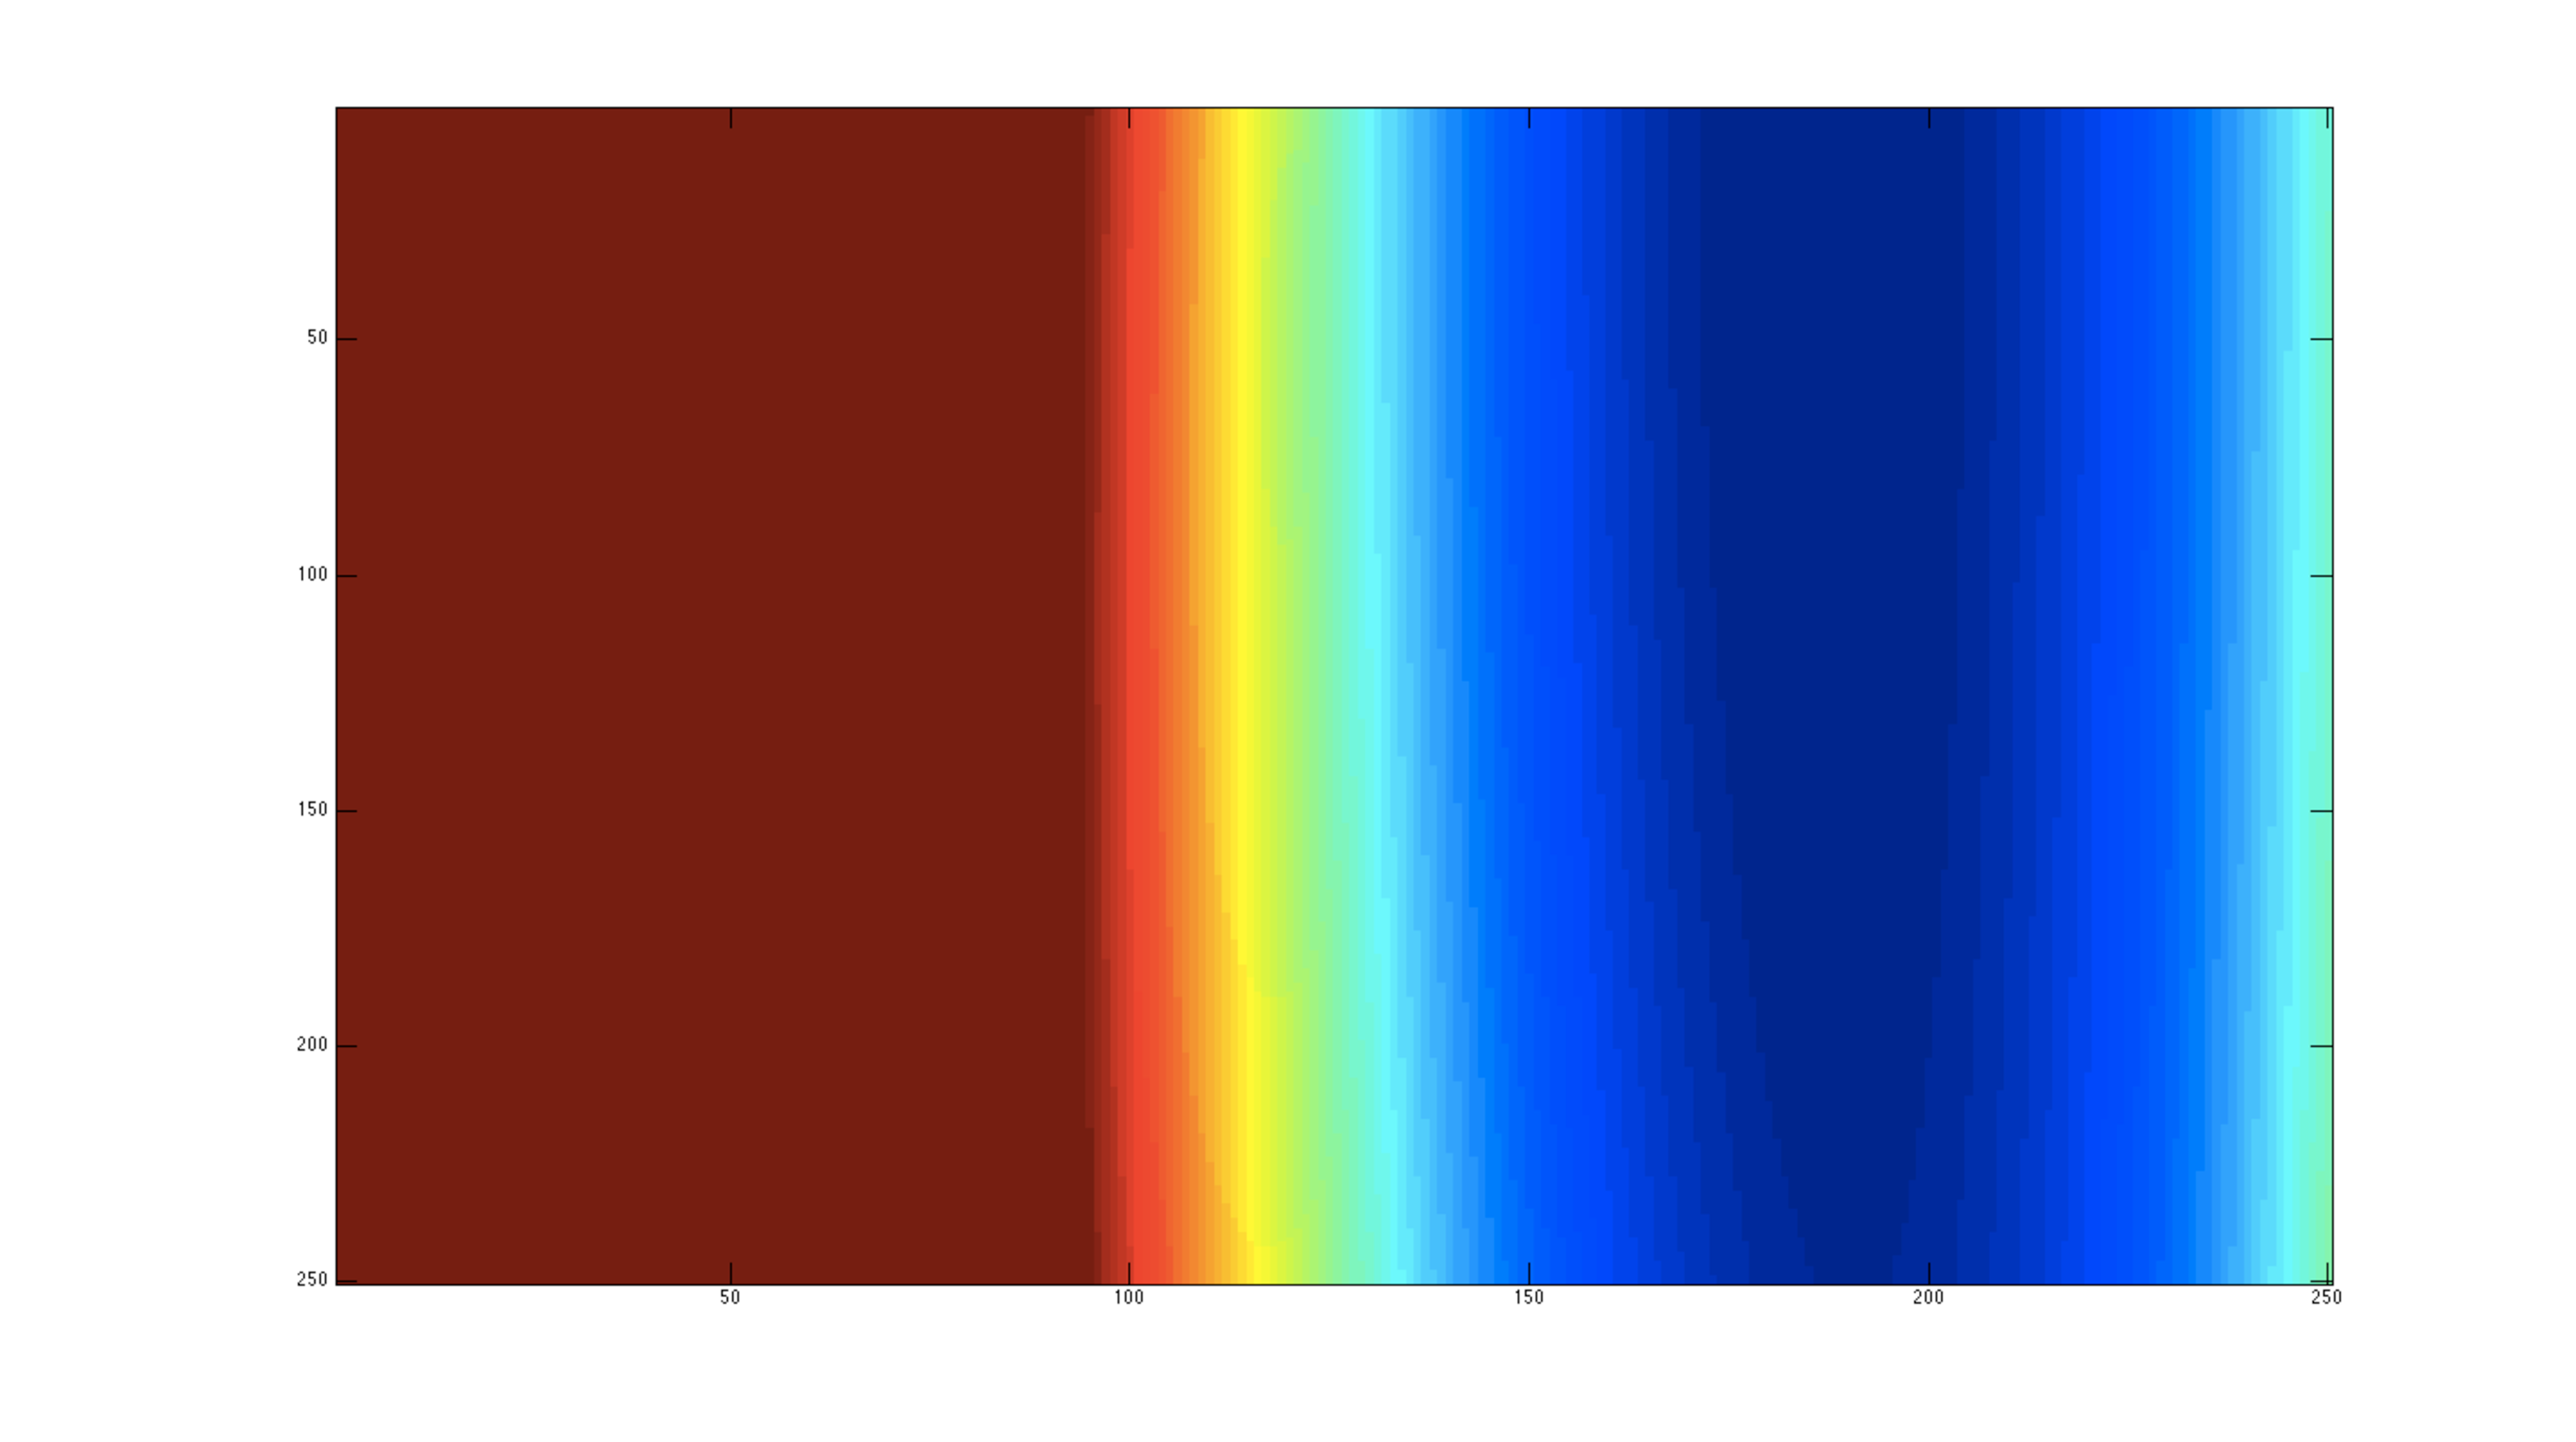
\includegraphics[width=\linewidth]{zagaris-ab-contours}
  \caption{$a$/$b$ plane colored by objective function value. Contours follow lines of constant $a$, the parameter affecting the geometry of the fast manifold.}
\end{figure}

\subsubsection{Nonlinear parameter transformation}

We can transform these stiff/sloppy pairs of $(\lambda, \epsilon)$ and $(a, b)$ using something like

\begin{align*}
  c_1 &= \sqrt{\frac{\epsilon}{E} + \frac{1}{S}\frac{\lambda}{L}} \cos(2\pi S \frac{\epsilon}{E}) \\
  c_2 &= \sqrt{\frac{\epsilon}{E} + \frac{1}{S}\frac{\lambda}{L}} \sin(2\pi S \frac{\epsilon}{E})
\end{align*}

for $\lambda \in [0, L]$ and $\epsilon \in [0, E]$. This will swirl the domain and produce nonlinear contours in $(c_1, c_2)$ space.

In the following figure, we have taken a set of sloppy parameters in the $\lambda$/$\epsilon$ plane and transformed them into a swirl in $c_1$/$c_2$. Subsequent application of DMAPS uncovers a parameterization of this nonlinear swirl as expected.

\begin{figure}[htbp]
  \centering
  \includegraphics[width=\linewidth]{c1-c2-dmap}
  \caption{DMAPS uncovers a parameterization of the nonlienarly transformed sloppy parameter set. Here the transformed parameter set is colored by the first DMAP eigenvector.}
\end{figure}

% \bibliographystyle{plain}
% \bibliography{literature.bib}

\end{document}
